\section{Analisi del prodotto}
	\subsection{Scopo del prodotto}
		Il capitolato C6 si pone come obiettivo creare una \glock{web-application} che permetta di analizzare grosse moli di dati ricevuti da sensori eterogenei tra loro. Tale applicazione mette a disposizione un'interfaccia che permette di visualizzare alcuni dati di interesse od eventuali correlazioni tra i dati stessi. Infine, per ogni tipologia di dato è possibile assegnarne il monitoraggio ad un particolare ente, ruolo o gruppo.
		
	\subsection{Analisi della struttura}
		La struttura del prodotto sarà divisa in:
		\begin{itemize}
			\item \textbf{Interfaccia di gestione}: L'interfaccia di gestione ed interrogazione permetterà agli utenti di seguire l'andamento di uno o più sensori, di controllarli, attivandoli o disattivandoli ed infine, agli utenti con maggiori privilegi, di aggiungere o rimuovere altri utenti o gruppi.
			Tramite questa interfaccia deve essere possibile inviare dei comandi al giusto gateway tramite un apposito \glock{topic} di Kafka per controllare gli \glock{edge data point}. 
			L'interfaccia di gestione dovrà dare la possibilità agli utenti di gestire i propri dati (quale ad esempio la password di accesso).
			\item \textbf{Database}: Si è pensato di utilizzare due tipi di database in base ai dati da memorizzare:
			\begin{itemize}
				\item Un database di tipo \glock{Time-Series} per memorizzare i dati temporali ricevuti dai sensori;
				\item Un database relazionale, per memorizzare i metadati relativi ai sensori (ad esempio il loro censimento) o relativi agli utenti che andranno ad utilizzare l'interfaccia di gestione.
			\end{itemize}

			\item \textbf{Gateway}: I dispositivi (o edge data point) che invieranno i dati dei loro sensori, non si interfacceranno direttamente con i database o con il cluster Kafka (descritto in seguito) bensì dialogheranno con un \glock{gateway} tramite degli appositi protocolli.
			Saranno presenti diversi gateway suddivisi per struttura, con almeno un gateway per sede, in modo tale da facilitare l'individuazione di uno specifico edge data point.
			Le configurazioni di invio dei dati (quale ad esempio la frequenza di invio) per ogni singolo dispositivo dovranno essere inviate dalla web app, che tramite un apposito topic di kafka, vengono salvate nell'apposito gateway, che poi si occuperà di filtrare i dati inviati dai dispositivi ed eventualmente trasformarli in formato JSON. 

			\item \textbf{Dispositivo (Edge Data Point)}: I dispositivi dopo essere stati censiti, invieranno dati al proprio gateway, senza essere consci della propria configurazione.

			\item \textbf{Cluster Apache Kafka}: Tramite Kafka e le sue API verranno ricevuti i dati dai sensori, passando da un gateway, verranno manipolati tramite degli stream ed infine salvati nel database e/o mostrati agli utenti che li richiedono. L'interfaccia di gestione ed il database contenente le misurazioni dei sensori si interfacceranno quindi con Kafka e non direttamente tra loro.

		\end{itemize}
	\subsection{Attori}

		\begin{figure}[t!]
			\centering
			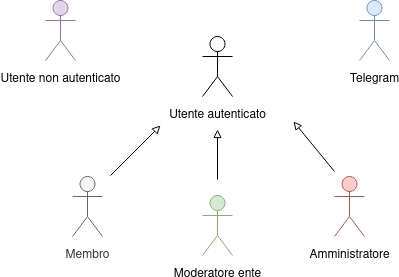
\includegraphics[scale=0.75]{res/images/attori}
			\caption{Diagramma riassuntivo degli attori con le relative generalizzazioni.}
		\end{figure}

		Gli attori individuati dopo un'attenta analisi del capitolato sono i seguenti:
		\subsubsection{Attori principali}
		\begin{itemize}
			\item \textbf{Utente non autenticato}: utente che non ha accesso alle sezioni private del sito poiché deve ancora eseguire l'autenticazione con le proprie credenziali. Inoltre, non ha ancora effettuato una prima autenticazione con il bot di \glock{Telegram}.

			\item \textbf{Utente autenticato}: utente che ha eseguito l'accesso al sito e ha accesso alle sezioni private del sito in base ai suoi permessi. Può gestire il proprio account attraverso le impostazioni e si è autenticato il bot di \glock{Telegram}. Si differenzia in tre tipologie:

			\begin{itemize}
				\item \textbf{Membro}: utente che può accedere alle sezioni del sito in base al suo ente di appartenenza. Questo tipo di utente deve appartenere a uno e un solo ente, ossia un gruppo che ha il permesso di visualizzare (in tabella o con un grafico) le misurazioni dei sensori. Può ricevere notifiche dal bot di \glock{Telegram}.

				\item \textbf{Moderatore ente}: Un moderatore ente ha tutti i permessi di un utente autorizzato e può gestire (visualizzare, modificare, rimuovere o aggiungere) i membri del proprio ente. Di questi ultimi, può visualizzare le relative attività (logs).
				Questo attore può impostare dei valori soglia, che quando superati provocano l'invio di notifiche a tutti i membri dell'ente.
				Possono essere presenti uno o più moderatori ente per ogni singolo ente.

				\item \textbf{Amministratore}: L'amministratore rappresenta un utente con il più alto livello di privilegi. Questo attore può infatti gestire (modificare, creare e rimuovere) gli enti, i loro membri e i dispositivi a loro assegnati. Non fa parte di un ente specifico, ma può visualizzare i dati di qualunque dispositivo censito. 
				L'amministratore può inoltre vedere tutte le attività di ogni singolo utente e può gestire l'invio della configurazione al gateway, decidendo quali dispositivi censire.
				Possono essere presenti uno o più amministratori generali.
			\end{itemize}
		\end{itemize}
		\subsubsection{Attori secondari}
			\begin{itemize}
				\item \glock{Telegram}: servizio di messaggistica istantanea che permette di realizzare \glock{Bot} che gestiscono invio e ricezione di messaggi da parte degli utenti. Attraverso questo servizio, si vuole gestire l'autenticazione a due fattori, l'invio di notifiche push e l'invio di comandi ai dispositivi remoti nel sistema.
			\end{itemize}
	